\documentclass{article} % For LaTeX2e
\usepackage{iclr2026_conference,times}

% Optional math commands from https://github.com/goodfeli/dlbook_notation.
\input{math_commands.tex}

\usepackage{hyperref}
\usepackage{url}
\usepackage{graphicx}
\usepackage{booktabs}
\usepackage{tabularx}
\usepackage{multirow}
\usepackage{amsmath,amssymb}

\title{StealthRL: Reinforcement Learning Paraphrase Attacks for\\
Multi-Detector Evasion of AI-Text Detectors}

\author{Anonymous Authors}

% \iclrfinalcopy % Uncomment for camera-ready version, but NOT for submission.
\begin{document}

\maketitle

\begin{abstract}
We introduce \emph{StealthRL}, a reinforcement-learning framework that paraphrases AI-generated text to evade detection while preserving meaning and fluency, enabling systematic red-teaming of AI-text detectors. The challenge is to reduce detector confidence at strict low-FPR operating points without collapsing semantic fidelity or overfitting to a single detector family. StealthRL fine-tunes a single Qwen3-4B paraphraser with LoRA \cite{hu2021loralowrankadaptationlarge} and a multi-objective reward combining detector evasion, semantic similarity, and fluency. On the MAGE benchmark with three detectors (RoBERTa OpenAI, Fast-DetectGPT, Binoculars), StealthRL reduces mean TPR@1\%FPR from 0.27 (no attack) to 0.04 while maintaining high semantic similarity (0.953 E5 cosine), outperforming simple paraphrasing and a detector-guided baseline. We release an anonymized code package in the supplementary material with a placeholder anonymous link for reproducibility.
\end{abstract}

\section{Introduction}
AI-generated text detectors are now embedded in academic integrity workflows, content moderation pipelines, and misinformation defenses. Yet detector robustness remains brittle under paraphrasing attacks: minor rewording can substantially reduce detection accuracy, especially at strict low-FPR thresholds that matter in high-stakes settings. This motivates red-teaming methodologies that generate high-fidelity paraphrases while systematically probing detector failure modes.

We focus on the adversarial aspect: generating paraphrases that evade multiple detector families without semantic drift. Existing evasion methods often optimize against a single detector or rely on prompt-only rephrasing, which may not generalize across detector families. We propose \textbf{StealthRL}, a reinforcement-learning paraphraser trained against a detector ensemble with explicit semantic and fluency constraints. The goal is not to enable misuse, but to provide reproducible stress tests that reveal detector fragility and guide defensive improvements.

\paragraph{Contributions.}
\begin{itemize}
  \item \textbf{Multi-detector RL paraphrasing.} We train a single paraphrase policy against a detector ensemble using group-relative policy optimization with LoRA, enabling efficient adversarial fine-tuning.
  \item \textbf{Low-FPR, transfer-aware evaluation.} We report attack success across detector families at TPR@1\%FPR with detector \(\times\) method heatmaps, tradeoff curves, and bootstrap confidence intervals.
  \item \textbf{Reproducible evaluation pipeline.} Our evaluation stack exports standardized per-sample scores, calibrated thresholds, and paper-ready figures, and supports MAGE with optional RAID and PadBen benchmarking. \cite{dugan2024raidsharedbenchmarkrobust,zha2025padben}
  \item \textbf{Plug-and-play training harness.} The training stack is modular (YAML-configurable detectors, rewards, and base models) and supports rapid ablations without code changes.
  \item \textbf{Empirical results.} On MAGE, StealthRL reduces mean TPR@1\%FPR to 0.04 (from 0.27 for no attack) while maintaining high semantic similarity.
\end{itemize}

\paragraph{Anonymized code release.}
An anonymized code release containing training and evaluation scripts is included in the supplementary material. A placeholder anonymous link is provided: \url{https://anonymous.4open.science/r/STEALTHRL}.

\section{Related Work}
\paragraph{AI-text detectors.} Curvature-based detectors such as DetectGPT and Fast-DetectGPT measure probability curvature under perturbations, while paired-LM detectors such as Binoculars compare base vs instruction-tuned likelihoods. \cite{mitchell2023detectgptzeroshotmachinegeneratedtext,bao2024fastdetectgptefficientzeroshotdetection,hans2024spottingllmsbinocularszeroshot} Classifier-based approaches (e.g., RoBERTa OpenAI, Ghostbuster) learn discriminative models and can be sensitive to domain shift. \cite{verma2024ghostbusterdetectingtextghostwritten}

\paragraph{Watermarking-based detection.} Watermarking approaches embed statistical signals into model outputs to enable reliable detection, forming a complementary detector family. \cite{kirchenbauer2023watermark} We focus on non-watermark detectors here, but watermark-aware evaluation is an important extension.

\paragraph{Adversarial paraphrasing.} Recent evasion methods use paraphrasing to reduce detector confidence, including Adversarial Paraphrasing and RL-based humanization such as AuthorMist. \cite{cheng2025adversarialparaphrasinguniversalattack,david2025authormistevadingaitext} These methods motivate our use of detector-guided rewards while highlighting the need for cross-detector transfer evaluation. Character-level attacks such as homoglyph substitutions demonstrate strong evasion but often degrade readability. \cite{creo2025silverspeakevadingaigeneratedtext}

\paragraph{Prompt-based and retrieval-aware evasion.} Krishna et al. show that paraphrasing substantially reduces detector accuracy and propose retrieval-based defenses. \cite{krishna2023paraphrasingevadesdetectorsaigenerated} Lu et al. demonstrate that large language models can be guided to evade detectors without model fine-tuning, highlighting the importance of robust evaluation under adaptive attacks. \cite{lu2024largelanguagemodelsguided} StealthRL complements these approaches by training a single RL policy that targets detector ensembles and evaluates transfer under low-FPR thresholds.

\paragraph{Evaluation benchmarks.} MAGE provides a standard benchmark for machine-generated text detection with diverse domains and generators, and is widely used in detector evaluation studies. \cite{li2024magemachinegeneratedtextdetection} RAID offers a large-scale robustness benchmark across domains and generators with stress tests for cross-domain generalization. \cite{dugan2024raidsharedbenchmarkrobust} PadBen focuses specifically on paraphrase attacks and includes tasks that probe multi-pass paraphrasing and attack depth. \cite{zha2025padben} We use MAGE as the primary evaluation benchmark in this work and report low-FPR operating point metrics consistent with prior evasion literature.

\section{Threat Model}
We assume \textbf{black-box access to detector scores}, i.e., the attacker can query detector confidence but does not require gradients. In practice, detectors are often open-source or deployed with a confidence API, so both black-box scoring and open-source replication are realistic. We evaluate transfer to a held-out detector family to test robustness beyond the training ensemble.

\section{Method}
Given AI-generated text $x$, we learn a paraphrase policy $\pi_\theta(y\mid x)$ that produces $y$ with low detector confidence while preserving meaning and fluency. We optimize a composite reward:
\begin{equation}
R(x,y) = \alpha R_{\text{det}}(y) + \beta R_{\text{sem}}(x,y) + \gamma R_{\text{ppl}}(y),
\end{equation}
where $R_{\text{det}}$ is the ensemble detector score (lower AI probability), $R_{\text{sem}}$ is E5 embedding cosine similarity, and $R_{\text{ppl}}$ is a fluency proxy derived from a frozen LM. We train with group-relative policy optimization (GRPO) and LoRA adapters \cite{hu2021loralowrankadaptationlarge} on Qwen/Qwen3-4B-Instruct-2507 (rank 32, $\alpha=32$, dropout 0.05). Training uses group size 4, learning rate $2.8\times10^{-4}$, batch size 16, and two epochs. The detector ensemble used for training is RoBERTa OpenAI + Fast-DetectGPT with weights 0.6/0.4.

\paragraph{Reward normalization and constraints.} Detector scores are z-score normalized online to stabilize the reward scale across training. Semantic similarity is thresholded at 0.90 and linearly mapped to $[0,1]$; fluency rewards are similarly thresholded with a minimum quality floor to avoid rewarding degenerate outputs. We also reject empty outputs and enforce length sanity checks (minimum length and upper bound relative to the source) to prevent collapse.

\paragraph{Optimization with GRPO.} GRPO computes advantages within a group of rollouts per prompt, avoiding a learned value model and reducing variance. We use group-normalized advantages and remove constant-reward groups to prevent degenerate updates. LoRA keeps the base LM frozen and updates only low-rank adapters, which is critical for efficient experimentation and stability.

\begin{figure}[t]
  \centering
  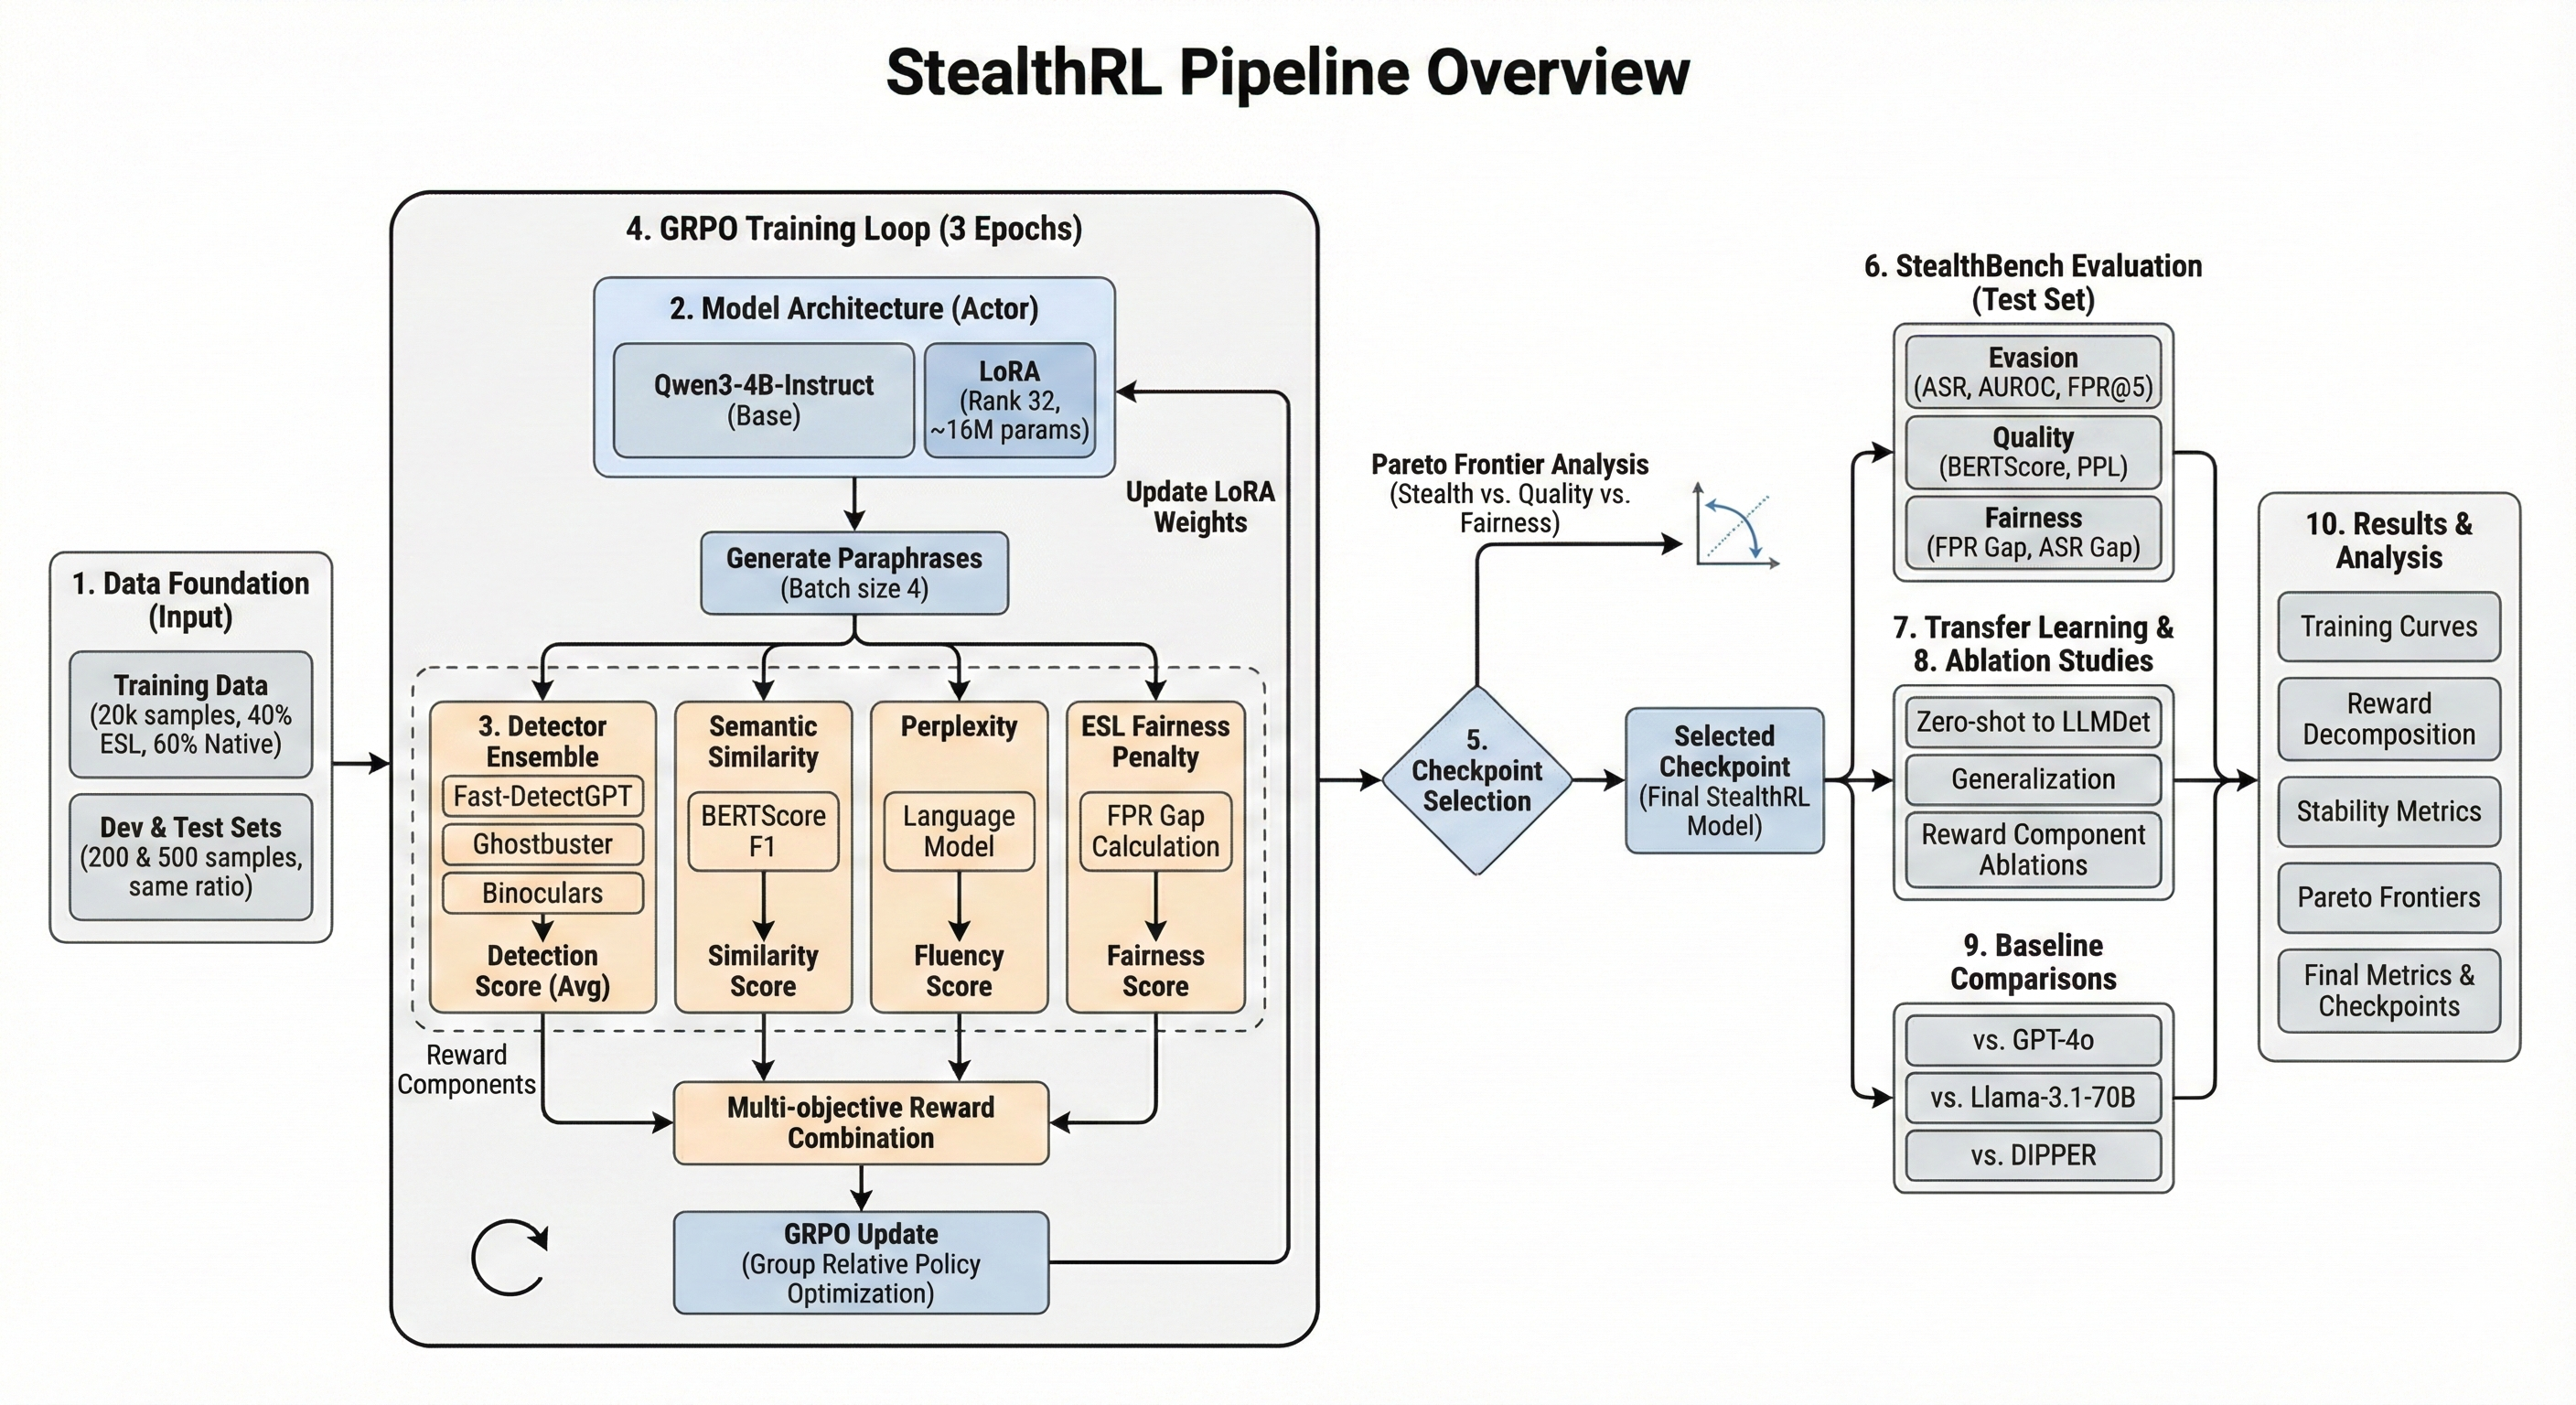
\includegraphics[width=\linewidth]{figures/StealthRL_Methodology.png}
  \caption{StealthRL training and evaluation pipeline. A single paraphrase policy is trained with detector-guided reward and quality constraints, then evaluated across multiple detector families with low-FPR metrics and tradeoff analysis.}
  \label{fig:pipeline}
\end{figure}

\section{Experimental Setup}
\paragraph{Dataset.} We evaluate on MAGE using the test split with 50 human and 50 AI samples, filtered to a 100--500 token window. \cite{li2024magemachinegeneratedtextdetection} The evaluation pipeline also supports RAID and PadBen for cross-benchmark generalization analysis; these are included as optional runs in the release. \cite{dugan2024raidsharedbenchmarkrobust,zha2025padben}

\paragraph{Detectors.} Evaluation uses three detector families: RoBERTa OpenAI classifier, Fast-DetectGPT (curvature-based), and Binoculars (paired-LM). \cite{mitchell2023detectgptzeroshotmachinegeneratedtext,bao2024fastdetectgptefficientzeroshotdetection,hans2024spottingllmsbinocularszeroshot}

\paragraph{Methods.} We compare six methods: M0 (no attack), M1 (simple paraphrase), M2 (StealthRL-v1 checkpoint), M3 (detector-guided selection inspired by Adversarial Paraphrasing), M4 (AuthorMist), and M5 (homoglyph substitution). \cite{cheng2025adversarialparaphrasinguniversalattack,david2025authormistevadingaitext,creo2025silverspeakevadingaigeneratedtext}

\paragraph{Metrics.} We calibrate a 1\% FPR threshold per detector on human texts and report TPR@1\%FPR (lower is better for the attacker), attack success rate (ASR = 1 - TPR@1\%FPR), and AUROC. We also report semantic similarity (E5 cosine) and text quality metrics. All results use one candidate per sample (n=1).

\section{Evaluation Protocol}
For each detector $d$, we compute a threshold $\tau_d$ such that the false positive rate on human texts is 1\%. We then evaluate AI samples using:
\begin{equation}
\text{TPR@1\%FPR}_d = \frac{1}{|\mathcal{A}|} \sum_{x \in \mathcal{A}} \mathbb{1}[s_d(x) > \tau_d],
\end{equation}
where $\mathcal{A}$ is the AI sample set and $s_d(x)$ is the detector score. The attack success rate is $\text{ASR}_d = 1 - \text{TPR@1\%FPR}_d$. We report mean TPR/ASR across detectors to summarize transfer, and AUROC as a detector separation metric. Bootstrap confidence intervals are computed in the evaluation pipeline (500 resamples) for per-detector metrics.
\begin{table}[t]
  \centering
  \small
  \begin{tabular}{l c}
\toprule
Detector & Threshold at 1\% FPR \\
\midrule
RoBERTa OpenAI & 0.574 \\
Fast-DetectGPT & 0.764 \\
Binoculars & 0.504 \\
\bottomrule
\end{tabular}

  \caption{Detector-specific thresholds calibrated at 1\% FPR on human texts (higher score indicates more likely AI).}
  \label{tab:thresholds}
\end{table}

\paragraph{Quality metrics.} We compute semantic similarity using E5 embeddings, chrF for surface-form preservation, and edit rate / token change rate to quantify transformation extent. A perplexity proxy from a frozen LM serves as a fluency indicator. These metrics are reported alongside detection evasion to capture the evasion--quality tradeoff.

\paragraph{LLM-based quality evaluation (optional).} Following Adversarial Paraphrasing, we optionally run an LLM autorater (GPT-5-mini) to score paraphrase quality and semantic equivalence on a 1--5 Likert scale, with a fixed per-method sample cap to control cost. This aligns with recent work on LLM-based automatic evaluators. \cite{cheng2025adversarialparaphrasinguniversalattack,vu2024foundationalautoraters,fu2023gptscore,kim2024prometheus2}

\section{Implementation and Reproducibility}
Training is implemented with a modular configuration system that defines the base model, reward weights, detectors, and optimization settings. The reward computation is asynchronous and caches detector scores to reduce repeated inference. During evaluation, we produce per-sample detector scores and per-method aggregates (including AUROC and low-FPR metrics) and export paper-ready figures and tables.

For reproducibility, the evaluation pipeline outputs (i) per-sample score tables, (ii) aggregated metrics with bootstrap confidence intervals, and (iii) standardized figures for detector transfer and quality tradeoffs. These artifacts are included in the anonymized code release and can be regenerated with a single evaluation command on the MAGE benchmark.

\section{Results}
Table~\ref{tab:main} summarizes detection evasion at 1\% FPR. StealthRL reduces mean TPR@1\%FPR to 0.04 (vs. 0.27 for no attack) and improves mean AUROC from 0.71 to 0.43. Per-detector TPR@1\%FPR drops from 0.22/0.28/0.32 (M0) to 0.08/0.02/0.02 (M2) on RoBERTa/Fast-DetectGPT/Binoculars, indicating transfer to the held-out detector family. StealthRL maintains high semantic similarity (0.953 E5 cosine), comparable to simple paraphrasing (0.959), while outperforming the detector-guided baseline (M3).

\begin{table}[t]
  \centering
  \small
  \setlength{\tabcolsep}{4pt}
  \begin{tabular}{lcccccc}
\toprule
Method & TPR@1\%FPR $\downarrow$ (R) & F (Fast) & B (Binoc) & Mean $\downarrow$ & ASR $\uparrow$ & AUROC $\downarrow$ \\
\midrule
M0 No Attack & 0.23 & 0.40 & 0.41 & 0.34 & 0.66 & 0.74 \\
M1 Simple Para & 0.10 & 0.10 & 0.04 & 0.08 & 0.92 & 0.59 \\
M2 StealthRL-v1 & \textbf{0.00} & \textbf{0.00} & \textbf{0.00} & \textbf{0.00} & \textbf{1.00} & \textbf{0.27} \\
M3 Adv. Para (guided) & 0.10 & 0.09 & 0.05 & 0.08 & 0.92 & 0.60 \\
M5 Homoglyph & \textbf{0.00} & \textbf{0.00} & \textbf{0.00} & \textbf{0.00} & \textbf{1.00} & 0.44 \\
\bottomrule
\end{tabular}

  \caption{Main results on MAGE (TPR@1\%FPR, ASR, and AUROC). Lower TPR/AUROC is better for the attacker; higher ASR is better. R/F/B denote RoBERTa/Fast-DetectGPT/Binoculars.}
  \label{tab:main}
\end{table}

\begin{figure}[t]
  \centering
  \includegraphics[width=0.92\linewidth]{figures/fig_heatmap_tpr.png}
  \caption{Detector \(\times\) method heatmap of TPR@1\%FPR. StealthRL shows consistently low TPR across detectors, indicating transfer beyond the training ensemble.}
  \label{fig:heatmap}
\end{figure}

\begin{figure}[t]
  \centering
  \includegraphics[width=0.85\linewidth]{figures/fig_tradeoff.png}
  \caption{Evasion--quality tradeoff (mean TPR@1\%FPR vs. semantic similarity). StealthRL achieves strong evasion while preserving meaning; homoglyph attacks improve evasion but degrade fluency and readability.}
  \label{fig:tradeoff}
\end{figure}

\begin{figure}[t]
  \centering
  \includegraphics[width=0.9\linewidth]{figures/fig_auroc_bars.png}
  \caption{Per-detector AUROC comparison across methods. Lower AUROC indicates weaker detector separation for the attacker.}
  \label{fig:auroc}
\end{figure}

\begin{figure}[t]
  \centering
  \includegraphics[width=0.9\linewidth]{figures/fig_method_comparison.png}
  \caption{Aggregate method comparison across detectors. StealthRL consistently outperforms simple paraphrasing and detector-guided selection under low-FPR thresholds.}
  \label{fig:method_cmp}
\end{figure}

\begin{figure}[t]
  \centering
  \includegraphics[width=0.9\linewidth]{figures/fig_score_distributions.png}
  \caption{Detector score distributions for human vs AI across methods. StealthRL shifts AI distributions toward human scores across detector families.}
  \label{fig:score_dist}
\end{figure}

\begin{figure}[t]
  \centering
  \includegraphics[width=0.9\linewidth]{figures/fig_human_ai_separation_roberta.png}
  \caption{Human vs AI score separation for the RoBERTa detector across methods. StealthRL reduces separability more than simple paraphrasing while maintaining fidelity.}
  \label{fig:roberta_sep}
\end{figure}

\begin{figure}[t]
  \centering
  \includegraphics[width=0.9\linewidth]{figures/fig_human_ai_separation_fast_detectgpt.png}\\
  \vspace{2pt}
  \includegraphics[width=0.9\linewidth]{figures/fig_human_ai_separation_binoculars.png}
  \caption{Human vs AI score separation for Fast-DetectGPT (top) and Binoculars (bottom) across methods. StealthRL shifts AI scores toward the human regime on both detectors, indicating transfer beyond the training ensemble.}
  \label{fig:sep_other}
\end{figure}

\begin{figure}[t]
  \centering
  \includegraphics[width=0.85\linewidth]{figures/fig_quality_vs_evasion.png}
  \caption{Quality vs evasion scatter. StealthRL balances semantic similarity and detector evasion across samples.}
  \label{fig:quality_evasion}
\end{figure}

\begin{table}[t]
  \centering
  \small
  \setlength{\tabcolsep}{4pt}
  \begin{tabular}{lcccc}
\toprule
Method & E5 Sim $\uparrow$ & PPL $\downarrow$ & EditRate $\uparrow$ & chrF $\uparrow$ \\
\midrule
M0 No Attack & 1.00 & 27.35 & 0.00 & 1.00 \\
M1 Simple Para & 0.96 & 31.09 & 0.83 & 0.56 \\
M2 StealthRL-v1 & 0.95 & 35.91 & 0.84 & 0.53 \\
M3 Adv. Para (guided) & 0.96 & 30.27 & 0.83 & 0.56 \\
M4 AuthorMist & 0.90 & 25.07 & 0.91 & 0.53 \\
M5 Homoglyph & 0.94 & 146.32 & 0.65 & 0.65 \\
\bottomrule
\end{tabular}
  \caption{Quality metrics on MAGE (E5 similarity, perplexity proxy, edit rate, chrF). Higher similarity and chrF are better; lower perplexity indicates more fluent outputs.}
  \label{tab:quality}
\end{table}

\paragraph{Score distributions and quality tradeoffs.} Figure~\ref{fig:score_dist} shows that StealthRL shifts AI score distributions toward the human regime across detectors. Figures~\ref{fig:roberta_sep} and \ref{fig:sep_other} visualize this effect per detector, with consistent separability reductions on the held-out families. Figure~\ref{fig:quality_evasion} highlights the expected tradeoff between evasion and fidelity. Homoglyph substitution achieves extremely low detection scores but at the cost of degraded fluency (high perplexity), while StealthRL maintains a balanced evasion--quality profile.

\paragraph{Ablation (implemented; results pending).} We implemented a \emph{guidance-transfer} ablation that mimics the ``guidance vs. deploy'' setting from Adversarial Paraphrasing: candidate selection is guided by (i) RoBERTa, (ii) Fast-DetectGPT, or (iii) the ensemble mean, and evaluated across all detectors. This isolates how guidance detector choice affects transfer. Results are pending for the final model checkpoints.

\paragraph{Qualitative examples.}
\begin{table}[h]
\centering
\small
\setlength{\tabcolsep}{4pt}
\begin{tabularx}{\linewidth}{X X}
\toprule
\textbf{Original (M0)} & \textbf{StealthRL (M2)} \\
\midrule
During cardio the heart increases its workload and all the body's other systems adjust to help support that endeavor. The blood vessels dilate, the muscles do their best to help pump blood back to the heart, and the lungs work harder to take in oxygen and remove waste gases like carbon dioxide. &
In cardio, the heart ramps up its workload, prompting the body's other systems to adapt and assist. Blood vessels widen, muscles strive to push blood back to the heart, and lungs intensify their efforts to absorb oxygen and expel waste gases such as carbon dioxide. \\
\midrule
The engine has to endure the torque of powering two axels and a drive shaft generally the transfer casing connects to the drive shaft with a ujoint and same for power distribution. The electricity goes into the battery first then is sent to the alternator where it generates voltage that powers all other electrical components like the lights, radio. &
The engine must handle the torque from two axles and a drive shaft, typically linked via a universal joint in the transfer casing for power distribution. Electricity first charges the battery, then flows to the alternator, which converts it into voltage to power essential electrical systems such as lights and the radio. \\
\bottomrule
\end{tabularx}
\caption{Representative paraphrases from the evaluation run (MAGE test split).}
\end{table}

\section{Limitations and Safety}
Our evaluation currently focuses on three detector families and one primary benchmark; additional detectors (e.g., watermark-based) and datasets can broaden coverage. Adversarial paraphrasing is dual-use: we present StealthRL as a red-teaming tool to expose detector fragility and inform defensive calibration, and we release code anonymized with the expectation of responsible use.

\section{LLM Usage Disclosure}
Large language models were used to assist with code scaffolding and with editing text for clarity. All modeling decisions, experiments, evaluations, and interpretations were designed, executed, and validated by the authors.

\section{Conclusion}
StealthRL provides a practical adversarial RL framework for generating high-fidelity paraphrases that evade multiple detector families under strict low-FPR constraints. Our results show strong transfer to a held-out detector while preserving semantic fidelity, and our released evaluation pipeline supports reproducible red-teaming of AI-text detectors.

\bibliographystyle{iclr2026_conference}
\bibliography{stealthrl_refs}

\end{document}
